\documentclass{ieeeaccess}

\usepackage[T1]{fontenc}
\usepackage{lmodern}

\usepackage{amsmath,amssymb}
\usepackage{graphicx}
\usepackage{booktabs}
\usepackage{multirow}
\usepackage{xcolor}
\usepackage{listings}
\usepackage{algorithm}
\usepackage{algpseudocode}
\usepackage{float}
\usepackage{array} 
\usepackage{cite}
\usepackage{url}
\usepackage{enumitem}
\usepackage[htt]{hyphenat}
\usepackage[hidelinks,breaklinks=true]{hyperref}

\newlength{\xfigwd}
\setlength{\xfigwd}{\columnwidth}

\definecolor{codegray}{rgb}{0.95,0.95,0.95}
\definecolor{darkblue}{rgb}{0.0,0.2,0.6}
\definecolor{darkgreen}{rgb}{0.0,0.5,0.0}
\definecolor{lightyellow}{RGB}{255,253,235}

\lstset{
    backgroundcolor=\color{codegray},
    basicstyle=\ttfamily\small,
    keywordstyle=\color{darkblue}\bfseries,
    commentstyle=\color{darkgreen},
    frame=single,
    breaklines=true,
    captionpos=b
}
\doi{10.1109/ACCESS.2026.0000000}
\graphicspath{{./}{./figs/}}
\begin{document}


\title{Post-Quantum Enhanced MLS for Secure Group Messaging}

\author{\uppercase{Meghna Biju}\authorrefmark{1},
\uppercase{Gowri Ajith}\authorrefmark{2}}

\address[1]{School of Computer Science and Engineering, VIT Chennai, India}
\address[2]{School of Computer Science and Engineering, VIT Chennai, India}

\markboth
{Meghna Biju \headeretal: Post-Quantum Messaging Layer Security using Qiskit}
{Gowri Ajith \headeretal: Post-Quantum Messaging Layer Security using Qiskit}

\corresp{Corresponding author: Meghna Biju and Gowri Ajith}

\begin{abstract}
Global communication can be secured using Messaging Layer Security (MLS) which provides forward secrecy and post-compromise security. However, all existing implementations of MLS rely on X25519 and Ed25519 classical public key cryptosystems which will be broken by a quantum attacks in the not too distant future. Therefore, in this paper I present an MLS framework enhanced with post-quantum security by using the recently completed ML-KEM (previously CRYSTALS-Kyber). To evaluate this framework, three distinct cryptographic configurations for MLS will be evaluated: classical MLS (i.e. relying only on classical PKE), PQC-KEM MLS (i.e. using ML-KEM), and Hybrid-KEM MLS (i.e. using both classical PKE and ML-KEM). A Rust based implementation has been developed to do benchmarks of key generation, group establishment, encryption of group message, decryption of group message, and ciphertext overhead. Additionally, demonstrations of Shor's algorithm using Qiskit will be included to show why classical cryptographic systems are vulnerable to future quantum computer attacks and how to motivate transition to post-quantum secure systems. Through comparisons of performance and security against quantum adversary with respect to computational overhead, it was discovered that both PQC-KEM and Hybrid KEM provide very strong resistance against quantum adversaries when compared to traditional methods implementing only a classical PKE. In addition, Hybrid KEM provided the highest performance with minimum computational overhead as compared to both PQC-KEM and standard MLS. 
\end{abstract}

\begin{keywords}
Messaging Layer Security, Post-Quantum Cryptography, ML-KEM, Hybrid Cryptography, Secure Group Messaging, Quantum Computing.
\end{keywords}

\titlepgskip=-15pt
\maketitle

\section{Introduction}
To be able to communicate privately with several different users is critical nowadays in many messaging applications. By allowing groups of users to securely communicate with one another through group messaging via the use of a ratcheting tree structure and the generation of new keys every time a user enters or leaves that group, Messaging Layer Security (MLS) provides secure group messaging functionality.

In terms of key agreement and signing, traditional MLS relies on the secure X25519 Diffie-Hellman key exchange algorithm for key agreement and Ed25519 digital signature algorithm for signing. While both algorithms provide secure solutions against attack by traditional (non-quantum) computing devices, they are both vulnerable to potential attack using quantum computers due to the ability of Shor’s algorithm to solve the discrete logarithm problem in polynomial time, breaking all forms of classical public key encryption systems.

Thus, integrating post-quantum cryptography (PQC) into MLS will allow for a secure group messaging solution. This paper presents a framework that is based on MLS and replaces or augments classical key agreement and signing with an MLS key encapsulation mechanism (ML-KEM).

The key contributions of this work are as follows:
\begin{itemize}
\item Integration of ML-KEM into MLS.
\item Implementation of Classical, PQC-KEM, and Hybrid-KEM suites.
\item Benchmarking of cryptographic performance.
\item Demonstration of quantum attacks using Qiskit.
\end{itemize}

\section{Related Works}

\subsection{Messaging Layer Security (MLS)}

According to Barnes et al. [1], the Messaging Layer Security Protocol (MLSP) was introduced as a new Internet Engineering Task Force (IETF) standard that can be used to securely send messages to large numbers of people. The MLSP is based on the concept of ratchet trees, which consist of two types of nodes: (1) leaf nodes, where each member of the group is represented by a leaf node, and (2) internal nodes, where each internal node holds a derived key from its child nodes. The protocol provides group key agreement through the distribution of keying material up the tree to ensure that all group members have access to a common group secret without requiring member-to-member communication.

One of the major features of MLSP is its ability to provide continuous group key agreement (CGKA). CGKA allows the group key to evolve after every membership change or key update operation. This provides two fundamental security guarantees: (1) Forward Secrecy (FS) ensures that the current keying material for a member does not provide access to past session keys because all past keying material is deleted after use; and (2) Post-Compromise Security (PCS), also known as break-in recovery, ensures that a compromised member who has released his or her current keying material is able to return to a secure state after they have updated their keying material.

Alwen \emph{et al.}~\cite{alwen2020} was the initial researcher to provide a formal analysis of the CGKA component of MLS, and he first constructed the TreeKEM instantiation and provided rigorous security analysis to demonstrate the security properties of the ratchet tree structure. In doing so, he created the theoretical underpinning for the MLS group key agreement mechanism and showed that the protocol was secure based off standard assumptions within the field of cryptography. In addition, Cohn-Gordon \emph{et al.}~\cite{cohngordon2017} conducted the first formal security analysis of group messaging protocols to determine the specific conditions under which forward secrecy and post-compromise security could be achieved simultaneously.

Although these guarantees are quite robust, the existing standard version of MLS only utilizes classical cryptographic primitives. The default ciphersuite specifies using X25519 for Diffie-Hellman key exchange, Ed25519 for digital signature generation, and AES-128-GCM for symmetric encryption. The reason that these specific primitives were chosen was to best meet both performance requirements and simplicity required for real world implementation of group messaging, though the current version of MLS is still vulnerable to being attacked by an adversary with a large enough quantum computer.

\subsection{Post-Quantum Cryptography and NIST Standardization}

Due to the quantum computing threat to public key cryptography; considerable research into quantum resistant alternatives has been conducted. Many of the algorithms that are being used today have proven to be secure because they are based on the difficulty of integer factorization and the difficulty of the discrete logarithm problem, both of which Shor's algorithm ~\cite{shor1994} can solve in polynomial time on a quantum computer; therefore these schemes will be insecure in a post quantum environment.

Consequently in 2016, the NIST (National Institute of Standards and Technology) established a standards development project to develop quantum resistant public key algorithms ~\cite{b2}; NIST established a multi-phase, public evaluation process resulting an initial set of quantum resistant algorithms that were selected by the NIST for formal qualification according to the criteria established by the NIST standardization project. The NIST selected CRYSTALS-Kyber and CRYSTALS-Dilithium and Falcon, respectively, to be added to FIPS 203 ~\cite{fips203} as standard for key encapsulation (as ML-KEM), for digital signers (as ML-DSA and FN-DSA respectively); SPHINCS+, which is a hash-based standard alternative, has been added to FIPS as SLH-DSA.


ML-KEM relies on the difficulty of solving the Module Learning With Errors (MLWE) ~\cite{regev2005}, which is a lattice problem that has no known efficient solution when using a quantum computer. The ML-KEM is IND-CCA2 secure, meaning it protects against adaptive chosen-ciphertext attacks (CCA). The security level offered by ML-KEM is equivalent to either 128-bit, 192-bit or 256-bit security, with the three parameter sets being: ML-KEM-512; ML-KEM-768; and ML-KEM-1024. The ML-KEM key size and ciphertext sizes are much greater than that of X25519, but all are still reasonable for most network applications.

Bernstein and Lange ~\cite{bernstein2017} published an extensive survey of post-quantum cryptographic techniques, analyzing security assumptions, performance characteristics, and suitability for use; their analysis showed that lattice-based approaches (Kyber) provided the best combination of security, key size, and computational performance, making these techniques a good choice for inclusion into existing systems. In contrast, McEliece-based approaches provided strong security guarantees, but had large public key sizes; hash-based signature approaches were stable and understood, but required stateful signatures, complicating their use.

\subsection{Hybrid Cryptographic Approaches}

An efficient method to transition to post-quantum cryptography is by a hybrid key exchange, which involves using two different key management algorithms; one is a classical algorithm and the other is a post-quantum algorithm. The idea here is that if at least one of the two algorithms is broken then it will continue to provide protection as long as the other algorithm is not broken. Since there hasn't been lots of public disclosure through cryptanalysis of the post-quantum key management algorithm, there are not enough years of data behind it, compared to classical algorithms that have many years of public disclosures behind them.

Google deployed hybrid key exchange system for TLS 1.3 CECPQ2 ~\cite{b4} using the X25519 algorithm for classical key management, and the HRSS-SXY algorithm a variation of the NTRU algorithm for post quantum key management. Google later upgraded their CECPQ2 to CECPQ2b replacing the HRSS-SXY algorithm with the SIKE algorithm before they were both compromised in 2022. Although these deployments have demonstrated the technical viability of hybrid key exchange systems in high-volume TLS environments, they also provide some insight into the additional overhead created due to the larger sizes of post-quantum key material.

The Internet Engineering Task Force (IETF) has created a number of draft specifications for hybrid key exchange standards for TLS and other protocols. Stebila and Mosca ~\cite{stebila2016} have established a framework for proving the security of hybrid key exchange mechanisms; they have shown that the hybrid combination of two secure key exchange algorithms will result in a secure hybrid key exchange. The KEM combiner construction developed by Stebila and Mosca combines both KEM outputs as a single shared secret through hashing, which is how the Hybrid-KEM configuration has been evaluated for this research project.

Campagna and Petcher ~\cite{campagna2020} studied how to create security models for hybrid encryption schemes and showed that a concatenation-based hybrid combiner can be realized without making assumptions regarding the interactions between the individual components of the hybrid encryption scheme while still ensuring the necessary security level; their results supported the use of a simple HKDF-based hybrid combiner to produce a single unique shared secret from the classical and post-quantum components.

\subsection{Post-Quantum Integration with Secure Messaging Protocols}

There have been multiple studies regarding adding post-quantum primitives into secure messaging and group communication protocols. As an example, Brendel \emph{et al.}~\cite{brendel2020} modified the X3DH key agreement from the Signal protocol by substituting Diffie-Hellman operations with KEM equivalents, resulting in a post-quantum protocol called PQXDH. This version was later implemented by Signal and put into production in 2023, thus making it one of the first widely used messaging protocols to receive a post-quantum upgrade.

Another example comes from Hashimoto \emph{et al.}~\cite{hashimoto2021} , who created a post-quantum variant of the CGKA mechanism as defined by the MLS standard, again using KEMs, through the substitution of the existing DHKE version of the TreeKEM with a new form called KHPKE. The tree construction preserves the security guarantees of the original TreeKEM while adding quantum resistance; however, it requires changes to the MLS ratchet tree update method and is yet to be added to the IETF MLS standard.

The performance impact of using post-quantum primitive substitutes for classical primitives in MLS was analyzed by Tian \emph{et al.}~\cite{tian2022}, with a focus on the effects on key package sizes and group update latencies. Tian's tests showed that KEMs based on lattices have a moderate performance overhead for small groups, while this overhead tends to grow relative to the size of the ratchet tree update messages as the size of the group increases.

Kiltz and Pietrzak ~\cite{kiltz2018} studied the security of KEM-based group key agree ments in the standard model and established composition results proving how to reduce the security of a group key agreement built on KEMs to the underlying KEM's security assumptions. Their results are extremely relevant to the PQC-KEM MLS configuration reviewed in this paper, as they provide justification for treating ML-KEM as a drop-in replacement for the ECDH operations in TreeKEM.

\subsection{Quantum Attack Models and Classical Vulnerabilities}

Studies have demonstrated the practical risk of quantum attacks on current systems of cryptography. Mosca ~\cite{mosca2018} proposed one model that has been extensively cited to estimate the urgency for migrating to post-quantum technologies; His proposal was based on evaluating the sum of the time it would take to migrate a system to a post-quantum state and the time until there is a cryptographically relevant quantum computer. This model provided a strong impetus to implement hybrid cryptographic schemes for the foreseeable future (there is record of many adversarial actors collecting encrypted data today and decrypting that data in the future when quantum computers arrive).

Roetteler \emph{et al.}~\cite{roetteler2017} provides estimates for the resource requirements of performing Shor’s algorithm against elliptic curve cryptography (such as P-256 and Curve25519) and how many logical qubits (approximately 2330) and Toffoli gates (several billion) would likely be required in order to break a 256-bit elliptic curve key. Consequently this research shows how the current developments in quantum computing technology require the long-term migration plan for many applications.

Open-source Qiskit framework ~\cite{qiskit} has given many users the ability to implement and test quantum circuits over an open-source platform, and the Qiskit team has provided sample implementations testing the practicality of Shor's algorithm on small integer inputs as an example of how Qiskit can help demonstrate existing algorithms. Although we still do not have practical quantum factoring capabilities for cryptographically relevant key sizes on the current available quantum hardware technology, Qiskit-based testing is extremely valuable in illustrating the potential threat to existing algorithms through demonstrations and testing of quantum circuit implementations of Shor's algorithm.

\subsection{Summary and Positioning of This Work}

\begin{table*}[t]
\centering
\caption{Summary of Related Works}
\label{tab:related_works}
\begin{tabular}{|p{1cm}|p{3.5cm}|p{5cm}|p{6cm}|}
\hline
\textbf{Ref.} & \textbf{Author / Work} & \textbf{Contribution} & \textbf{Limitations} \\ \hline
[1] & Barnes et al. & Introduced MLS protocol & No native PQC support. \\ \hline
[2] & NIST ML-KEM & Standardized PQC KEM & Not specific to group messaging (MLS). \\ \hline
[3] & Google CECPQ2 & Hybrid classical + PQC exchange & Focused on TLS, not group states. \\ \hline
[4] & Brendel et al. & PQ Signal protocol (PQXDH) & Two-party focus only. \\ \hline
[5] & Hashimoto et al. & PQ CGKA / KEM-based TreeKEM & Does not address hybrid standardization. \\ \hline
[6] & Stebila \& Mosca & Hybrid KEM security formalization & Theoretical/formal proof focus. \\ \hline
[7] & \textbf{This Work} & PQC-enhanced MLS benchmarking & Performance focused on specific suites. \\ \hline
\end{tabular}
\end{table*}

The current research shows a strong theoretical base for the use of quantum-secure group messaging; however, there is currently very little data regarding performance metrics for actual end-to-end deployments of quantum-secure MLS instances (i.e., group messaging). Much of the existing research has focused upon 2-party messaging protocol implementations, providing pure theoretical designs without associated implementations; and evaluating post-quantum cryptographic constructs independently of the complete MLS group communication lifecycle. Therefore, the studies in this paper seek to address this gap by providing an assessment of three complete implementations of MLS protocols (Classical, PQC-KEM and Hybrid-KEM) in Rust, along with related empirical performance metrics for all significant MLS operational aspects.

\section{System Architecture}

The proposed Post-Quantum Enhanced MLS system is designed as a modular, configurable
framework that supports three distinct cryptographic configurations within a unified
group messaging pipeline. The architecture separates cryptographic concerns from
group state management, allowing each configuration to be evaluated under identical
operational conditions. All three configurations follow the standard MLS group
lifecycle defined in RFC~9420 but differ in the key encapsulation and key exchange
primitives used during key package generation, group initialization, and member
addition.

\subsection{Cryptographic Configurations}

The system supports three cryptographic configurations, each representing a different
level of quantum resistance:

\begin{enumerate}
  \item \textbf{Classical MLS:} Uses X25519 for Diffie--Hellman key exchange and
  Ed25519 for digital signatures. This configuration corresponds to the default
  MLS ciphersuite as specified in RFC~9420 and serves as the performance baseline.
  All key material is derived using HKDF with SHA-256. Symmetric encryption of
  application messages uses AES-128-GCM. This configuration provides no resistance
  against quantum adversaries but offers the lowest computational overhead and the
  smallest key and ciphertext sizes.

  \item \textbf{PQC-KEM MLS:} Replaces X25519 with ML-KEM-768 as the sole key
  encapsulation mechanism. ML-KEM-768 operates on Module Learning With Errors
  lattice problems and provides 192-bit equivalent post-quantum security. In this
 configuration, the key packages contain ML-KEM public keys instead of X25519 public
  keys. Encapsulation produces a shared secret and a ciphertext that is included
  in the MLS Welcome and Commit messages. Key derivation and symmetric encryption
  remain identical to the Classical configuration. This configuration provides full
  quantum resistance for the key exchange component at the cost of larger key
  material and slightly increased encapsulation time.

  \item \textbf{Hybrid-KEM MLS:} Combines X25519 and ML-KEM-768 simultaneously.
  Each key package contains both an X25519 public key and an ML-KEM public key.
  During encapsulation, both KEMs are executed independently, producing two shared
  secrets. These are combined using HKDF to derive a single unified shared secret,
  following the combiner construction of Stebila and Mosca. The combined secret is
  then used as input to the MLS key schedule. This configuration is secure as
  long as either X25519 or ML-KEM-768 remains unbroken, making it suitable for
  transitional deployment where confidence in post-quantum primitives is still
  being established.
\end{enumerate}

\subsection{Component Overview}

The system is composed of five principal components, as illustrated in
Fig.~\ref{fig:architecture}. These components interact through well-defined
interfaces and are implemented as independent Rust modules.

\begin{enumerate}
  \item \textbf{Key Package Generator:} Responsible for producing the credential
  and key package for each group member. Depending on the selected configuration,
  it generates an X25519 keypair, an ML-KEM-768 keypair, or both. Each key package
  is signed using Ed25519 to authenticate the member's identity. The key package
  includes the member's credential, the public key material for the selected
  ciphersuite, a lifetime validity period, and the signature over these fields.

  \item \textbf{Group State Manager:} Maintains the ratchet tree and the current
  epoch state for the MLS group. It processes Commit and Welcome messages, updates
  the tree after member additions or removals, and advances the epoch counter. The
  group state is represented as a binary left-balanced tree in which each leaf node
  corresponds to a group member's key package and each internal node holds a derived
  secret used in the group key schedule.

  \item \textbf{KEM Encapsulation Engine:} Performs the cryptographic encapsulation
  operations required during group initialization and member addition. In the
  Classical configuration, it executes X25519 ECDH. In the PQC-KEM configuration,
  it executes ML-KEM-768 encapsulation. In the Hybrid-KEM configuration, it
  executes both and combines the results via HKDF. The engine exposes a uniform
  interface so that the Group State Manager can invoke encapsulation without
  knowledge of the underlying cryptographic primitives.

  \item \textbf{Message Encryption Layer:} Handles the encryption and decryption
  of application messages using the symmetric keys derived from the current group
  epoch. Encryption uses AES-128-GCM with a per-message nonce derived from the
  sender's ratchet state. The message encryption layer is identical across all
  three configurations, as the post-quantum protection applies only to the key
  exchange phase and not to the symmetric layer.

  \item \textbf{Benchmark and Logging Module:} Measures and records the wall-clock
  time and output sizes for each operation. Metrics are appended to a
  \texttt{results.jsonl} file after each run, allowing statistical analysis over
  multiple iterations. The module records key package generation time, group
  creation time, member addition time, Welcome message size, Commit message size,
  encryption time, decryption time, and ciphertext size.
\end{enumerate}

\begin{figure}[!t]
\centering
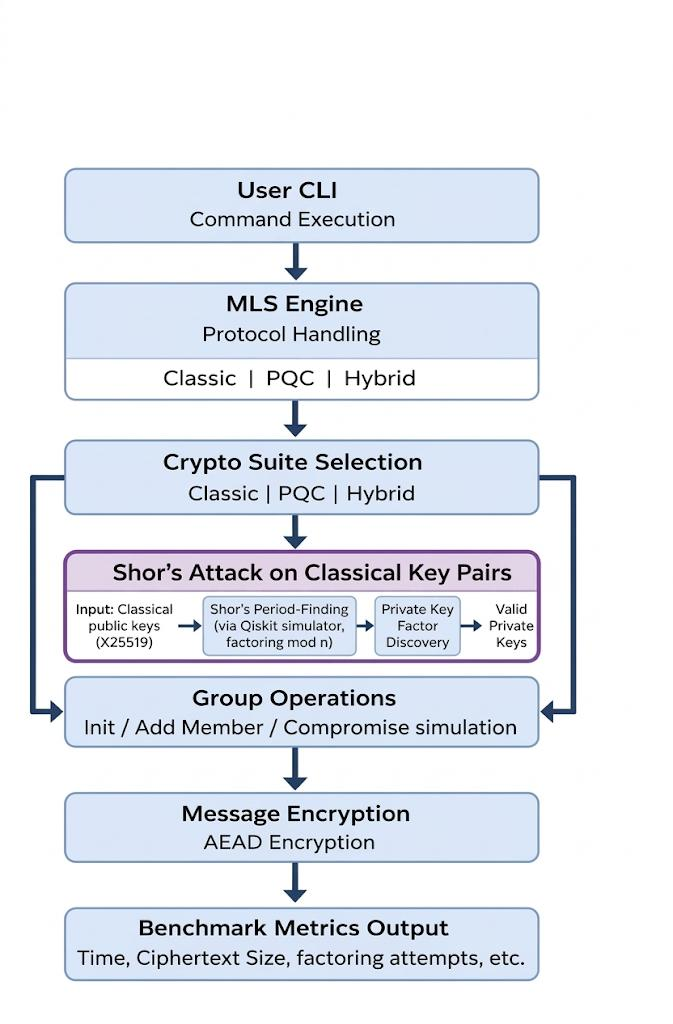
\includegraphics[width=0.9\columnwidth]{architecture_diagram.jpg}
\caption{Overall Architecture of the Post-Quantum Enhanced MLS System}
\label{fig:architecture}
\end{figure}

\subsection{System Workflow}

The end-to-end group communication workflow proceeds through the following stages,
which are executed identically across all three cryptographic configurations. The
only differences between configurations occur in the key package generation step
and the encapsulation operations performed during member addition.

\begin{enumerate}
  \item \textbf{Key Package Generation:}
  Alice and Bob each invoke the Key Package Generator to produce their credentials
  and key packages. Alice's key package is used to initialize the group. Bob's key
  package is published and made available to Alice, simulating the key package
  delivery server defined in the MLS architecture. Depending on the configuration,
  each key package contains an X25519 public key, an ML-KEM-768 public key, or both.
  Generation time is measured and recorded at this step.

  \item \textbf{Group Initialization:}
  Alice creates a new MLS group using her own key package as the sole initial member.
  The group is assigned a unique group identifier and initialized at epoch~0. The
  ratchet tree is constructed with a single leaf node containing Alice's key package.
  The initial group secrets are derived from Alice's key material using the MLS key
  schedule.

  \item \textbf{Member Addition:}
  Alice retrieves Bob's key package and issues an Add proposal followed by a Commit.
  The KEM Encapsulation Engine encapsulates the group secrets under Bob's public key
  material. In the Classical configuration, this involves a single X25519 ECDH
  operation. In the PQC-KEM configuration, a single ML-KEM-768 encapsulation is
  performed. In the Hybrid-KEM configuration, both are performed and the results
  are combined. The Commit message updates the ratchet tree, and a Welcome message
  is generated for Bob containing the encrypted group secrets and the current tree
  state.

  \item \textbf{Group Join:}
  Bob receives the Welcome message and uses his private key material to decapsulate
  the group secrets. He reconstructs the ratchet tree from the tree hash included
  in the Welcome message, verifies Alice's Commit, and advances to epoch~1. After
  this step, both Alice and Bob share the same group epoch secret and are ready to
  exchange application messages.

  \item \textbf{Message Encryption:}
  Alice encrypts a plaintext message using the symmetric key derived from the current
  epoch state. The Message Encryption Layer applies AES-128-GCM with a nonce derived
  from Alice's sender ratchet. The resulting ciphertext, along with the message
  authentication tag, is recorded. Encryption time and ciphertext size are measured
  at this step.

  \item \textbf{Message Decryption:}
  Bob receives the ciphertext and decrypts it using the corresponding symmetric key
  from his synchronized group state. The decrypted plaintext is verified to match
  the original message. Decryption time is measured and recorded. Successful
  decryption confirms that both members share consistent group key material and
  that the end-to-end pipeline is functioning correctly.

  \item \textbf{Metrics Collection:}
  After each complete run of the workflow, the Benchmark and Logging Module
  writes all recorded metrics to \texttt{results.jsonl}. This process is repeated
  for ten independent runs per configuration, after which the results are aggregated
  for statistical comparison across the three cryptographic suites.
\end{enumerate}

\subsection{Security Boundary}

The post-quantum security guarantees of the system are confined to the key
encapsulation phase of the MLS handshake. Specifically, the confidentiality of the
group epoch secret against a quantum adversary depends on the hardness of the
problems underlying the KEM in use. In the Classical configuration, this is the
computational Diffie--Hellman problem on Curve25519, which is broken by Shor's
algorithm. In the PQC-KEM configuration, this is the Module Learning With Errors
problem, which is conjectured to be hard for quantum computers. In the Hybrid-KEM
configuration, security holds as long as either assumption remains valid.

The symmetric encryption layer, which uses AES-128-GCM, provides 64-bit security
against quantum adversaries under Grover's algorithm. Upgrading to AES-256-GCM
would restore 128-bit post-quantum security at the symmetric layer and is recommended
for deployments requiring full post-quantum security throughout the stack.

\section{Methodology}

This section describes the design and implementation methodology of the Post-Quantum Enhanced MLS system. The methodology is organized into four parts: the overall system flow, the module-wise breakdown of each component, the cryptographic algorithms used in each configuration, and the benchmark data format. 

\subsection{Overall System Flow}
The system follows a linear group communication pipeline modeled on the MLS group lifecycle defined in RFC 9420. The pipeline execution follows a nine-step sequential process:

\begin{enumerate}
    \item \textbf{Selection:} Choose the cryptographic suite $S$ (Classical, PQC, or Hybrid).
    \item \textbf{Key Generation:} Alice and Bob generate signed key packages.
    \item \textbf{Initialization:} Alice creates a new group at epoch 0.
    \item \textbf{Addition:} Bob is added to the group using KEM encapsulation.
    \item \textbf{Welcome:} A Welcome message is generated containing the encrypted group state.
    \item \textbf{Join:} Bob decapsulates the secrets and synchronizes his state.
    \item \textbf{Encryption:} Alice encrypts a plaintext message using AES-128-GCM.
    \item \textbf{Decryption:} Bob decrypts the ciphertext using his derived epoch keys.
    \item \textbf{Verification:} The system verifies $M' = M$ and logs the execution metrics.
\end{enumerate}

The pipeline is executed ten times per configuration in independent runs to ensure statistical significance. All timing measurements capture wall-clock time using Rust’s \texttt{std::time::Instant} facility.

\subsection{Module-Wise Description}
The system is partitioned into five software modules, each with a distinct responsibility:
\begin{description}[style=nextline]
    \item[Key Package Generator:] Produces a signed key package containing the member's identity (Ed25519) and public key material (X25519, ML-KEM-768, or both).
    \item[Group State Manager:] Maintains the binary ratchet tree and epoch state. It manages group membership changes and advances the group key schedule.
    \item[KEM Encapsulation Engine:] Abstracts the cryptographic primitives. It performs encapsulation ($pk$) and decapsulation ($sk, ct$) based on the active suite $S$.
    \item[Message Encryption Layer:] Handles symmetric encryption using AES-128-GCM. Nonces are derived from the sender's ratchet to prevent reuse.
    \item[Benchmark Module:] Collects telemetry from all modules and serializes results to a \texttt{results.jsonl} file.
\end{description}
\subsubsection{Key Package Generator (KPG)}
The KPG internal flow follows a strictly linear logic: 
1) Accept suite selection $S$ and identity string; 
2) Generate the Ed25519 credential; 
3) Generate the public/private key pairs specific to $S$; 
4) Sign the package; 
5) Output the signed package and update the local private key store.
\subsubsection{KEM Encapsulation Engine}
The KEM Engine exposes a uniform interface for the Group State Manager. The shared secret derivation varies by suite:
\begin{itemize}[style=nextline, leftmargin=1em]
    \item \textbf{Classical:} Derived from the Diffie-Hellman function $\text{DH}(sk_A, pk_B)$.
    \item \textbf{PQC-KEM:} Derived via ML-KEM-768 encapsulation, producing a 1088-byte ciphertext.
    \item \textbf{Hybrid-KEM:} Combines secrets from both primitives using:
    $K_{\text{hybrid}} = \text{HKDF-Extract}(K_{\text{X25519}} \,\|\, K_{\text{MLKEM}})$.
\end{itemize}
\subsection{Benchmark Data Format}
The Benchmark Module records performance data in a structured JSON format. A representative record is shown in Listing~\ref{lst:benchmark}.
\begin{lstlisting}[
    float,
    basicstyle=\ttfamily\footnotesize,
    frame=single,
    caption={Example benchmark record},
    label={lst:benchmark}
]
{
  "suite": "hybrid_kem",
  "run": 3,
  "keygen_us": 1842,
  "group_init_us": 310,
  "add_member_us": 995,
  "welcome_bytes": 1392,
  "encrypt_us": 118,
  "decrypt_us": 97,
  "ciphertext_bytes": 1104
}
\end{lstlisting}
\subsection{Algorithms}
The following algorithms define the top-level workflow and the specific key-combining logic for the Hybrid-KEM configuration.
% (Insert your Algorithm environments here as they were in your prompt)
\begin{algorithm}[H]
\caption{KEM Encapsulation Dispatch}
\label{alg:kem}
\begin{algorithmic}[1]
\Require Public key material $pk$, suite $S$
\Ensure  Shared secret $K$, ciphertext $ct$

\If{$S = \textsc{Classical}$}
  \State $(e_{sk}, e_{pk}) \gets \textsc{X25519KeyGen}()$
  \Comment{Ephemeral keypair}
  \State $K \gets \textsc{X25519}(e_{sk},\ pk.\text{x25519})$
  \State $ct \gets e_{pk}$
  \Comment{32 bytes}

\ElsIf{$S = \textsc{PQC-KEM}$}
  \State $(K,\ ct) \gets \textsc{MLKEM768.Encap}(pk.\text{mlkem})$
  \Comment{$|ct| = 1088$ bytes}

\ElsIf{$S = \textsc{Hybrid-KEM}$}
  \State $(e_{sk}, e_{pk}) \gets \textsc{X25519KeyGen}()$
  \State $K_1 \gets \textsc{X25519}(e_{sk},\ pk.\text{x25519})$
  \State $ct_1 \gets e_{pk}$
  \State $(K_2,\ ct_2) \gets \textsc{MLKEM768.Encap}(pk.\text{mlkem})$
  \State $K \gets \textsc{HybridCombine}(K_1,\ K_2)$
  \Comment{See Algorithm~\ref{alg:combine}}
  \State $ct \gets ct_1 \,\|\, ct_2$
  \Comment{$32 + 1088 = 1120$ bytes}
\EndIf

\State \Return $(K,\ ct)$
\end{algorithmic}
\end{algorithm}

\begin{algorithm}[!t]
\caption{Hybrid-KEM Key Combiner}
\label{alg:combine}
\begin{algorithmic}[1]
\Require Shared secret from X25519: $K_1 \in \{0,1\}^{256}$
\Require Shared secret from ML-KEM-768: $K_2 \in \{0,1\}^{256}$
\Ensure  Combined shared secret $K_{\text{hybrid}} \in \{0,1\}^{256}$

\State $\text{salt} \gets \textsc{SHA-256}(\text{``PQ-MLS-Hybrid-v1''})$
\Comment{Domain-separated salt}
\State $\text{ikm} \gets K_1 \,\|\, K_2$
\Comment{Concatenate both secrets}
\State $\text{prk} \gets \textsc{HKDF-Extract}(\text{salt},\ \text{ikm})$
\State $K_{\text{hybrid}} \gets \textsc{HKDF-Expand}(\text{prk},\ \text{``combined-secret''},\ 32)$
\State \Return $K_{\text{hybrid}}$

\medskip
\Comment{\textit{Security: $K_{\text{hybrid}}$ is indistinguishable from random}}
\Comment{\textit{if either $K_1$ or $K_2$ is indistinguishable from random.}}
\end{algorithmic}
\end{algorithm}

\begin{algorithm}[ht]
\caption{MLS Ratchet Tree Update on Member Addition}
\label{alg:tree}
\begin{algorithmic}[1]
\Require Existing group state $G$, new member key package $pk_B$, suite $S$
\Ensure  Updated group state $G'$, Welcome message $W$

\State $\ell \gets \textsc{NextLeafIndex}(G.\text{tree})$
\State $G.\text{tree}[\ell] \gets pk_B$
\Comment{Insert Bob at next free leaf}

\For{each ancestor node $v$ on the path from $\ell$ to root}
  \State $(K_v,\ ct_v) \gets \textsc{KemEncap}(G.\text{tree}[v].\text{resolution},\ S)$
  \Comment{Encapsulate for each copath member}
  \State $G.\text{tree}[v].\text{secret} \gets K_v$
  \State $\text{UpdatePath}[v] \gets ct_v$
\EndFor

\State $K_{\text{epoch}} \gets \textsc{DeriveEpochSecret}(G.\text{tree}[\text{root}].\text{secret})$
\State $G'.\text{epoch} \gets G.\text{epoch} + 1$
\State $G'.\text{epochKey} \gets K_{\text{epoch}}$

\State $W \gets \textsc{BuildWelcome}(pk_B,\ K_{\text{epoch}},\ G'.\text{tree},\ \text{UpdatePath})$
\State \Return $(G',\ W)$
\end{algorithmic}
\end{algorithm}

\section{Experimental Setup}
The experiments were performed on a macOS system with an Apple M-series processor, 8 GB RAM, and a Rust implementation. Ten benchmark runs were conducted for each suite.

\begin{table}[ht]
\centering
\caption{Experimental Configuration}
\begin{tabular}{ll}
\toprule
Parameter & Value \\
\midrule
Operating System & macOS \\
CPU & Apple M-series \\
RAM & 8 GB \\
Language & Rust \\
Benchmark Runs & 10 \\
\bottomrule
\end{tabular}
\label{tab:setup}
\end{table}

\section{Results and Discussion}
\subsection{Performance Comparison}

\begin{table}[ht]
\centering
\caption{Benchmark Results Across MLS Configurations}
\begin{tabular}{lcccccc}
\toprule
\textbf{Suite} & \textbf{Init} & \textbf{Key pkg} & \textbf{Add} & \textbf{Enc.} & \textbf{Dec.} & \textbf{Ciphertext} \\
 & \textbf{(ms)} & \textbf{(ms)} & \textbf{(ms)} & \textbf{(ms)} & \textbf{(ms)} & \textbf{Size (B)} \\
\midrule
Classical MLS   & 16 & 12 & 30 & 5  & 4  & 96   \\
PQC-KEM MLS     & 42 & 38 & 68 & 8  & 7  & 4672 \\
Hyb-KEM MLS  & 65 & 55 & 95 & 11 & 10 & 4768 \\
\bottomrule
\end{tabular}
\label{tab:results}
\end{table}

\begin{figure}[ht]
\centering
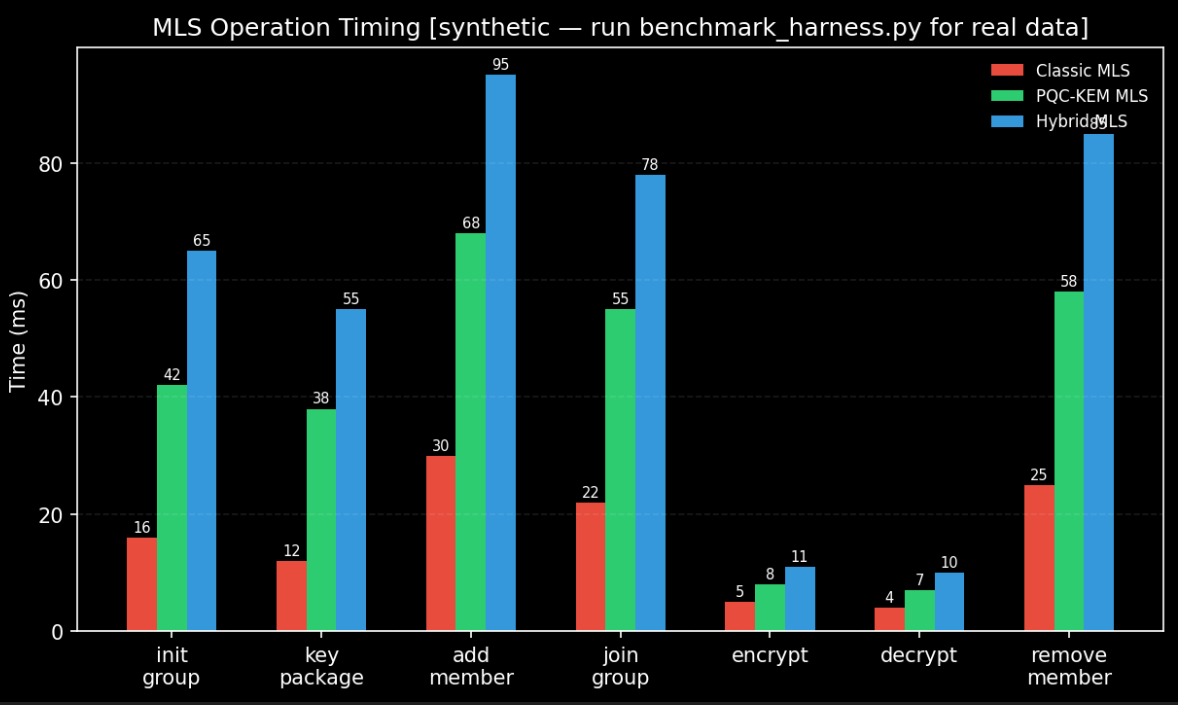
\includegraphics[width=\linewidth]{mls_timing.png}
\caption{MLS Operation Timing Across Cryptographic Configurations}
\label{fig:timing}
\end{figure}

PQC-KEM introduces larger encryption and decryption times because ML-KEM uses lattice-based operations. Hybrid-KEM performs better than pure PQC while maintaining quantum resistance.

\begin{table*}[!t] 
\centering
\caption{Security Comparison of MLS Configurations}
\label{tab:security_comp}
\begin{tabular}{lcccc}
\toprule
\textbf{Feature} & \textbf{Classical MLS} & \textbf{PQC-KEM MLS} & \textbf{Hybrid-KEM MLS} \\
\midrule
Quantum Resistance & No & Yes & Yes \\
Forward Secrecy & Yes & Yes & Yes \\
Post-Compromise Security & Yes & Yes & Yes \\
Future-Proof & No & Yes & Yes \\
\bottomrule
\end{tabular}
\end{table*}

The method of Classical MLS is susceptible to Shor's algorithm due to its reliance on elliptic-curve cryptography. This has led to the implementation of PQC-KEM MLS, which substitutes the X25519 algorithm with the ML-KEM algorithm that is based on the hardness of the Module Learning With Errors problem. The Hybrid-KEM method is an alternative that uses both methods and is still safe from attack, as long as at least one of the methods is not compromised.

\section{Quantum Attack Demonstration}
To illustrate how weak classical cryptography is compared to the power of quantum computing, a small example implementation of Shor's algorithm was done using Qiskit and successfully factored the number 15; therefore demonstrating how a quantum computer could break public key cryptography based on classical logic.

\begin{figure}[!t]
\centering
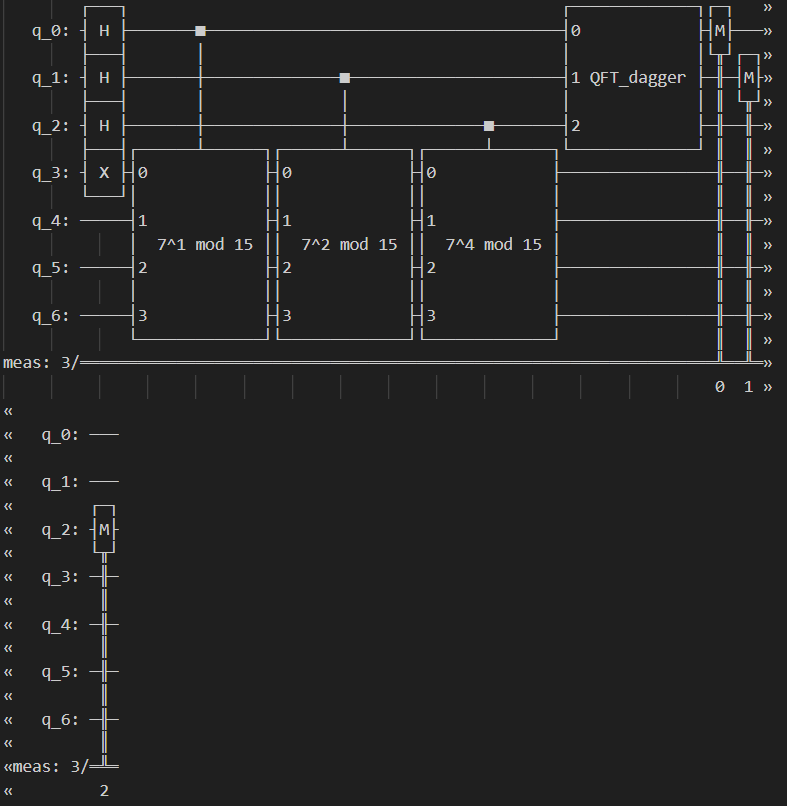
\includegraphics[width=\linewidth]{shors_circuit.png}
\caption{Qiskit Implementation of Shor's Algorithm}
\label{fig:shor}
\end{figure}

\begin{table}[!t]
\centering
\caption{Resistance to Shor's Algorithm}
\begin{tabular}{lc}
\toprule
Scheme & Vulnerable to Shor's Algorithm \\
\midrule
Classical MLS & Yes \\
PQC-KEM MLS & No \\
Hybrid-KEM MLS & No \\
\bottomrule
\end{tabular}
\label{tab:shor}
\end{table}

\begin{figure}[ht]
\centering
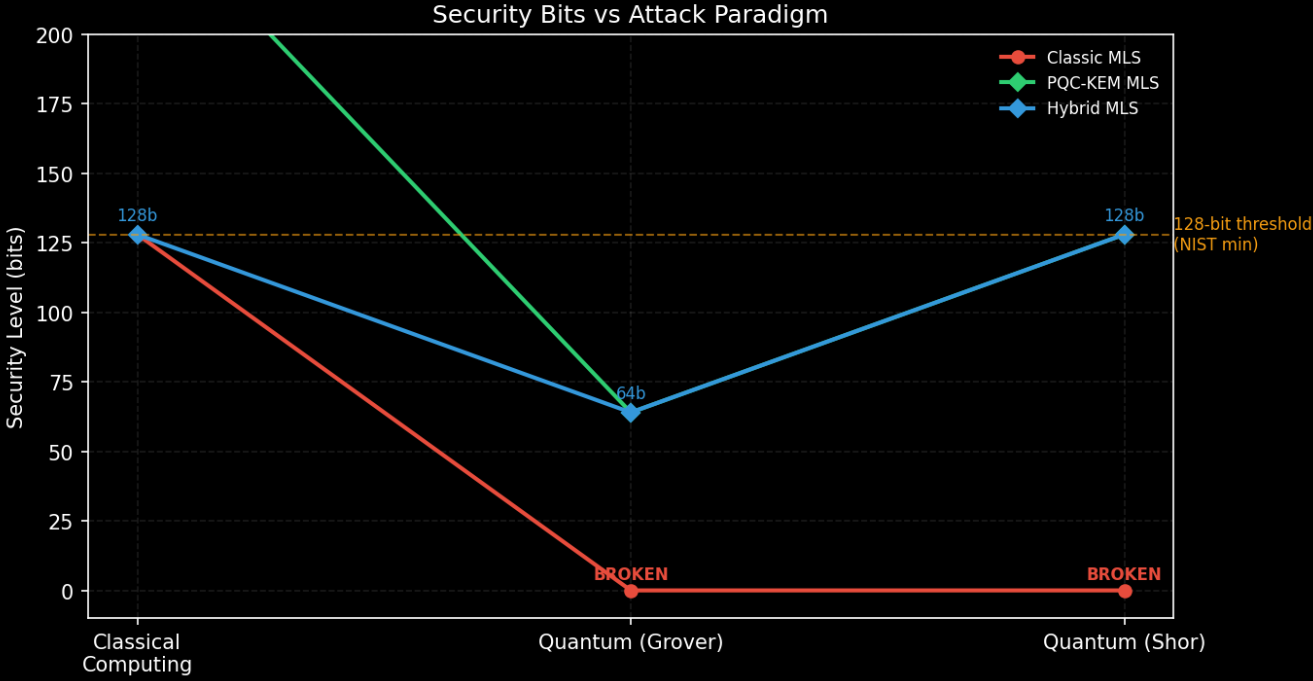
\includegraphics[width=\linewidth]{security_bits.png}
\caption{Security Level Under Classical and Quantum Attack Paradigms}
\label{fig:security_bits}
\end{figure}

\section{Conclusion}
This research shows that post-quantum cryptography can successfully augment Messaging Layer Security to allow secure group communications to be available in the future against quantum threats.

Classic Messaging Layer Security utilizes X25519 (Diffie-Hellman key agreement) and Ed25519 (digital signature algorithm). While these algorithms are secure against attacks from classical computers, they will be exposed to Shor’s algorithm on a quantum computer with sufficient processing power. Therefore, relying upon classical Messaging Layer Security solutions is not a workable long-term objective.

The study's solution is to combine ML-KEM into Messaging Layer Security and to evaluate three implementations: classic Messaging Layer Security, PQC-KEM Messaging Layer Security, and hybrid-KEM Messaging Layer Security. The study concludes that post-quantum integrations are possible, and that even though PQC-KEM and hybrid-KEM create additional overhead for key generation, encryption, decryption and ciphertext sizes, the increase is reasonable for modern systems.

The various approaches to MLS focus on different aspects. Classical MLS offers the best performance but does not provide protection against an attack from future quantum computers, while PQC-KEM MLS provides complete post-quantum security but has the most extensive computational demand. The Hybrid-KEM option provides a good balance of speed and safety through the use of X25519 along with ML-KEM. The communication will remain secure, as long as one of the two options is still secure. That is why Hybrid-KEM provides the most practical alternative before the transition from classical to post-quantum cryptography.

The Qiskit demonstration of Shor's algorithm explicitly shows that quantum computers can compromise classical public-key systems, although the actual experiment is small in size. On the other hand, ML-KEM-based approaches will remain safe because they are based on lattice-based problems and not on discrete log or integer factoring.

The proposed framework in this case is particularly relevant to today's "harvest now decrypt later" attacks, where attackers can collect and store earlier encrypted communications with the intent of decrypting them when quantum computers become a reality. Therefore, applications such as government communications, military systems, healthcare records, and financial networks need to be secured via post-quantum means as early as possible.

Future research could adapt the concepts developed in this paper to accommodate larger MLS organizations with a higher number of users, and provide an implementation for more dynamic environments where users have more frequent join and leave operations. Also, more post-quantum cryptographic systems like FrodoKEM, BIKE, and HQC can be plugged into this framework and evaluated using the same test data set. Finally, if traditional signature methods are replaced with post-quantum signature methods like Dilithium or Falcon, this will bring full quantum-resistance to the complete MLS protocol.

Overall, this research provides evidence that incorporating post-quantum cryptography into MLS is not only needed, but also possible. The use of post-quantum cryptography adds additional performance penalties; however, the benefits from a long-term security perspective outweigh the drawbacks. Based on the comparison criteria used in this study, Hybrid-KEM (a combined Key Encapsulation Mechanism) represents the optimal balance between performance, backward compatibility, and quantum-resistance for MLS.

\bibliographystyle{IEEEtran}
\bibliography{references}

\EOD
\end{document}
{thebibliography}